\documentclass[addpoints,12pt]{exam}\usepackage[]{graphicx}\usepackage[]{color}
%% maxwidth is the original width if it is less than linewidth
%% otherwise use linewidth (to make sure the graphics do not exceed the margin)
\makeatletter
\def\maxwidth{ %
  \ifdim\Gin@nat@width>\linewidth
    \linewidth
  \else
    \Gin@nat@width
  \fi
}
\makeatother

\definecolor{fgcolor}{rgb}{0.345, 0.345, 0.345}
\newcommand{\hlnum}[1]{\textcolor[rgb]{0.686,0.059,0.569}{#1}}%
\newcommand{\hlstr}[1]{\textcolor[rgb]{0.192,0.494,0.8}{#1}}%
\newcommand{\hlcom}[1]{\textcolor[rgb]{0.678,0.584,0.686}{\textit{#1}}}%
\newcommand{\hlopt}[1]{\textcolor[rgb]{0,0,0}{#1}}%
\newcommand{\hlstd}[1]{\textcolor[rgb]{0.345,0.345,0.345}{#1}}%
\newcommand{\hlkwa}[1]{\textcolor[rgb]{0.161,0.373,0.58}{\textbf{#1}}}%
\newcommand{\hlkwb}[1]{\textcolor[rgb]{0.69,0.353,0.396}{#1}}%
\newcommand{\hlkwc}[1]{\textcolor[rgb]{0.333,0.667,0.333}{#1}}%
\newcommand{\hlkwd}[1]{\textcolor[rgb]{0.737,0.353,0.396}{\textbf{#1}}}%
\let\hlipl\hlkwb


\makeatletter
\newenvironment{kframe}{%
 \def\at@end@of@kframe{}%
 \ifinner\ifhmode%
  \def\at@end@of@kframe{\end{minipage}}%
  \begin{minipage}{\columnwidth}%
 \fi\fi%
 \def\FrameCommand##1{\hskip\@totalleftmargin \hskip-\fboxsep
 \colorbox{shadecolor}{##1}\hskip-\fboxsep
     % There is no \\@totalrightmargin, so:
     \hskip-\linewidth \hskip-\@totalleftmargin \hskip\columnwidth}%
 \MakeFramed {\advance\hsize-\width
   \@totalleftmargin\z@ \linewidth\hsize
   \@setminipage}}%
 {\par\unskip\endMakeFramed%
 \at@end@of@kframe}
\makeatother

\definecolor{shadecolor}{rgb}{.97, .97, .97}
\definecolor{messagecolor}{rgb}{0, 0, 0}
\definecolor{warningcolor}{rgb}{1, 0, 1}
\definecolor{errorcolor}{rgb}{1, 0, 0}
\newenvironment{knitrout}{}{} % an empty environment to be redefined in TeX

\usepackage{alltt}
\usepackage{amsmath, amssymb}
\linespread{1.1}
\usepackage{hyperref}
\usepackage{enumerate}
\usepackage{multirow}
\usepackage{enumitem}

%-------------------DON'T CHANGE---------------------%
%The following is needed to prevent a conflict between knitr and the exam class involving the package ``framed.''



%This keeps images from being too big, centers them, and makes sure we use pdf images



%Change the default width of the output to fit within the solution boxes

%-------------------DON'T CHANGE---------------------%

%\printanswers

\title{Problem Set \# 11}
\author{Econ 103}
\date{}
\IfFileExists{upquote.sty}{\usepackage{upquote}}{}
\begin{document}
\maketitle

\section*{Lecture Progress}
We made it to slide 72 of the Chapter 8 slides.

\section*{Homework Checklist}

\begin{itemize}[label = $\square$]
	\item \textbf{Book Problems (Chapter 9):} 7, 9, 11, 23, 25, 27, 29
	\item \textbf{Additional Problems: }See below
	\item \textbf{Ask questions on Piazza}
	\item\textbf{Review slides}
	\item\textbf{R Tutorial:} Develop testable hypotheses for your R project and test at least one of them.
\end{itemize}

\section*{Additional Problems}

\begin{questions}

\question This problem uses a dataset that investigates the relationship between schizophrenia and the volume (in cm$^3$) of a particular region of the brain (the left hippocampus) measured using an MRI machine. 

The dataset contains 15 sets of monozygotic (i.e.\ identical) twins, one of whom has schizophrenia (``Affected'') and the other who does not (``Unaffected''). The idea of using identical twins is to hold constant unobserved genetic and socioeconomic confounding variables that might influence whether someone develops schizophrenia. You can download the data from Professor DiTraglia's website as follows:
\begin{knitrout}
\definecolor{shadecolor}{rgb}{0.969, 0.969, 0.969}\color{fgcolor}\begin{kframe}
\begin{alltt}
\hlstd{data.url} \hlkwb{<-} \hlstr{"http://www.ditraglia.com/econ103/case0202.csv"}
\hlstd{twins} \hlkwb{<-} \hlkwd{read.csv}\hlstd{(data.url)}
\hlkwd{head}\hlstd{(twins)}
\end{alltt}
\begin{verbatim}
##   Unaffected Affected
## 1       1.94     1.27
## 2       1.44     1.63
## 3       1.56     1.47
## 4       1.58     1.39
## 5       2.06     1.93
## 6       1.66     1.26
\end{verbatim}
\end{kframe}
\end{knitrout}
For this question you may assume that the sample differences between the left hippocampus volume of the ``Affected'' and ``Unaffected'' twins are drawn from a normal population with unknown variance.
	\begin{parts}
	\part Carry out a one-sided test at the 5\% level of the null hypothesis of no difference against the alternative that the affected twin has a larger left hippocampus, on average. What is your test statistic? What is your critical value? What is your decision rule? What is your decision?
  \begin{solution}
  First load the data and calculate the quantities we'll need to carry out all of the tests below.
\begin{knitrout}
\definecolor{shadecolor}{rgb}{0.969, 0.969, 0.969}\color{fgcolor}\begin{kframe}
\begin{alltt}
\hlstd{twin.diff} \hlkwb{<-} \hlstd{twins}\hlopt{$}\hlstd{Unaffected} \hlopt{-} \hlstd{twins}\hlopt{$}\hlstd{Affected}
\hlstd{mean.diff} \hlkwb{<-} \hlkwd{mean}\hlstd{(twin.diff)}
\hlstd{n.twins} \hlkwb{<-} \hlkwd{length}\hlstd{(twin.diff)}
\hlstd{SE.paired} \hlkwb{<-} \hlkwd{sqrt}\hlstd{(}\hlkwd{var}\hlstd{(twin.diff)}\hlopt{/}\hlstd{n.twins)}
\end{alltt}
\end{kframe}
\end{knitrout}
Notice that we calculated the differences as Unaffected twin minus Affected twin. We need to be careful about the sign here to see when we should reject the null. In this part, we are testing against the one-sided alternative that the \emph{Affected} twin has a larger left hippocampus. Thus, we should reject when \texttt{twin.diff} is \emph{sufficiently negative}. Now we calculate the test statistic and critical value for the one-sided test:
\begin{knitrout}
\definecolor{shadecolor}{rgb}{0.969, 0.969, 0.969}\color{fgcolor}\begin{kframe}
\begin{alltt}
\hlstd{test.stat} \hlkwb{<-} \hlstd{mean.diff}\hlopt{/}\hlstd{SE.paired}
\hlstd{test.stat}
\end{alltt}
\begin{verbatim}
## [1] 3.228928
\end{verbatim}
\begin{alltt}
\hlstd{critical.value} \hlkwb{<-} \hlkwd{qt}\hlstd{(}\hlnum{0.05}\hlstd{,} \hlkwc{df} \hlstd{= n.twins} \hlopt{-} \hlnum{1}\hlstd{)}
\hlstd{critical.value}
\end{alltt}
\begin{verbatim}
## [1] -1.76131
\end{verbatim}
\begin{alltt}
\hlstd{test.stat} \hlopt{<=} \hlstd{critical.value}
\end{alltt}
\begin{verbatim}
## [1] FALSE
\end{verbatim}
\end{kframe}
\end{knitrout}
In this case, our decision rule is to reject the null if the test statistic is \emph{less than} -1.7613101. (Remember, we have to keep track of the sign.) We see that this is not the case, so we fail to reject the null. We have not found evidence that the Affected twin has a larger left hippocampus.
  \end{solution}
	\part Repeat part (a) for a test against the \emph{opposite} one-sided alternative.
    \begin{solution}
    The test statistic remains the same in this case, but our decision rule and critical value have changed. Again, note that we calculated the differences as Unaffected twin minus Affected twin. Thus, a large \emph{positive} value of \texttt{mean.diff} would provide evidence that we should reject the null in favor of the one-sided alternative that the Unaffected twin has the larger left hippocampus, on average. The critical value simply changes sign to reflect this:
\begin{knitrout}
\definecolor{shadecolor}{rgb}{0.969, 0.969, 0.969}\color{fgcolor}\begin{kframe}
\begin{alltt}
\hlstd{critical.value} \hlkwb{<-} \hlkwd{qt}\hlstd{(}\hlnum{1} \hlopt{-} \hlnum{0.05}\hlstd{,} \hlkwc{df} \hlstd{= n.twins} \hlopt{-} \hlnum{1}\hlstd{)}
\hlstd{critical.value}
\end{alltt}
\begin{verbatim}
## [1] 1.76131
\end{verbatim}
\begin{alltt}
\hlstd{test.stat} \hlopt{>=} \hlstd{critical.value}
\end{alltt}
\begin{verbatim}
## [1] TRUE
\end{verbatim}
\end{kframe}
\end{knitrout}
  Our decision rule is to reject when the test statistic is greater than or equal to 1.7613101. Since this is the case, we reject the null hypothesis that the difference is zero at the 5\% significance level. We have found evidence that schizophrenia is associated with a smaller left hippocampus based on the twin data. 
    \end{solution}
	\part Repeat part (a) but test against the \emph{two-sided} alternative.
    \begin{solution}
      Again, the test statistic remains the same. Since we're testing against the two-sided alternative, however, we reject if it is too large \emph{or} two small. This is equivalent to asking whether the \emph{absolute value} of the test statistic is larger than the appropriate (positive) two-sided critical value:
\begin{knitrout}
\definecolor{shadecolor}{rgb}{0.969, 0.969, 0.969}\color{fgcolor}\begin{kframe}
\begin{alltt}
\hlstd{critical.value}  \hlkwb{<-} \hlkwd{qt}\hlstd{(}\hlnum{1} \hlopt{-} \hlnum{0.05}\hlopt{/}\hlnum{2}\hlstd{,} \hlkwc{df} \hlstd{= n.twins} \hlopt{-} \hlnum{1}\hlstd{)}
\hlstd{critical.value}
\end{alltt}
\begin{verbatim}
## [1] 2.144787
\end{verbatim}
\begin{alltt}
\hlkwd{abs}\hlstd{(test.stat)} \hlopt{>=} \hlstd{critical.value}
\end{alltt}
\begin{verbatim}
## [1] TRUE
\end{verbatim}
\end{kframe}
\end{knitrout}
We see that this is indeed the case, so we would reject that null hypothesis that the difference is zero against the two-sided alternative at the 5\% significance level.
    \end{solution}
	\part Explain the differences between your results in parts (a), (b), and (c).
    \begin{solution}
    Both parts (b) and parts (c) give the same result: reject the null. Parts (a) and (b) are mutually exclusive: if we reject in favor of one of the one-sided alternatives, we can't reject in favor of the other. This is because the \texttt{mean.diff} is either positive or negative: if positive, it suggests that the Unaffected twin has a larger left hippocampus; if negative, that the Affected twin does. We saw in class that, in borderline cases, it is possible to reject against a one-sided alternative without rejecting against the two-sided alternative. We are not in such a situation here.
    \end{solution}
	\part Calculate the p-values corresponding to parts (b) and (c).
    \begin{solution}
\begin{knitrout}
\definecolor{shadecolor}{rgb}{0.969, 0.969, 0.969}\color{fgcolor}\begin{kframe}
\begin{alltt}
\hlnum{1} \hlopt{-} \hlkwd{pt}\hlstd{(test.stat,} \hlkwc{df} \hlstd{= n.twins} \hlopt{-} \hlnum{1}\hlstd{)}
\end{alltt}
\begin{verbatim}
## [1] 0.003030772
\end{verbatim}
\begin{alltt}
\hlnum{2} \hlopt{*} \hlstd{(}\hlnum{1} \hlopt{-} \hlkwd{pt}\hlstd{(}\hlkwd{abs}\hlstd{(test.stat),} \hlkwc{df} \hlstd{= n.twins} \hlopt{-} \hlnum{1}\hlstd{))}
\end{alltt}
\begin{verbatim}
## [1] 0.006061544
\end{verbatim}
\end{kframe}
\end{knitrout}
  We see that both the one-sided p-value for part (b) and the two-sided p-value for (c) are quite small: there is extremely strong evidence against the null hypothesis of no difference. From these values, for example, we see that we would have still rejected if we had carried out these two tests at the 1\% rather than the 5\% level.
    \end{solution}
	\end{parts}
	


\question This problem concerns a dataset comparing the scores of men and women on the Armed Forces Qualifying Test (AFQT). Throughout you may assume that the sample size is large enough for the CLT to apply. As before, the data are available from Professor DiTraglia's website:
\begin{knitrout}
\definecolor{shadecolor}{rgb}{0.969, 0.969, 0.969}\color{fgcolor}\begin{kframe}
\begin{alltt}
\hlstd{data.url} \hlkwb{<-} \hlstr{"http://www.ditraglia.com/econ103/ex0222.csv"}
\hlstd{test.scores} \hlkwb{<-} \hlkwd{read.csv}\hlstd{(data.url)}
\hlkwd{head}\hlstd{(test.scores)}
\end{alltt}
\begin{verbatim}
##   Gender Arith Word Parag Math AFQT
## 1   male    19   27    14   14 70.3
## 2 female    23   34    11   20 60.4
## 3   male    30   35    14   25 98.3
## 4 female    30   35    13   21 84.7
## 5 female    13   30    11   12 44.5
## 6 female     8   15     6    4  4.0
\end{verbatim}
\end{kframe}
\end{knitrout}
Each row is an individual who took the test. The first column gives that individual's sex, while the second through fifth columns give the individual's score on four parts of the test. The final column is an overall percentile score for the test. 
	\begin{parts}
		\part For each section of the exam, as well as for overall percentile scores, test the null hypothesis that the population mean scores are equal for men and women at the 5\% level. In which cases do you reject, and in which cases do you fail to reject? 
    \begin{solution}
    First load the data and calculate the quantities we'll need to carry out the tests.
\begin{knitrout}
\definecolor{shadecolor}{rgb}{0.969, 0.969, 0.969}\color{fgcolor}\begin{kframe}
\begin{alltt}
\hlstd{test.men} \hlkwb{<-} \hlkwd{subset}\hlstd{(test.scores, Gender} \hlopt{==} \hlstr{'male'}\hlstd{)[,}\hlopt{-}\hlnum{1}\hlstd{]}
\hlstd{means.men} \hlkwb{<-} \hlkwd{apply}\hlstd{(test.men,} \hlnum{2}\hlstd{, mean)}
\hlstd{var.men} \hlkwb{<-} \hlkwd{apply}\hlstd{(test.men,} \hlnum{2}\hlstd{, var)}
\hlstd{n.men} \hlkwb{<-} \hlkwd{nrow}\hlstd{(test.men)}
\hlstd{test.women} \hlkwb{<-}\hlkwd{subset}\hlstd{(test.scores, Gender} \hlopt{==} \hlstr{'female'}\hlstd{)[,}\hlopt{-}\hlnum{1}\hlstd{]}
\hlstd{means.women} \hlkwb{<-} \hlkwd{apply}\hlstd{(test.women,} \hlnum{2}\hlstd{, mean)}
\hlstd{var.women} \hlkwb{<-} \hlkwd{apply}\hlstd{(test.women,} \hlnum{2}\hlstd{, var)}
\hlstd{n.women} \hlkwb{<-} \hlkwd{nrow}\hlstd{(test.women)}
\hlstd{diff.means} \hlkwb{<-} \hlstd{means.men} \hlopt{-} \hlstd{means.women}
\hlstd{SE} \hlkwb{<-} \hlkwd{sqrt}\hlstd{(var.women}\hlopt{/}\hlstd{n.women} \hlopt{+} \hlstd{var.men}\hlopt{/}\hlstd{n.men)}
\end{alltt}
\end{kframe}
\end{knitrout}
Since we've arranged the differences of means and associated standard errors in \emph{vectors}, we can calculate all of the test statistics at once!
\begin{knitrout}
\definecolor{shadecolor}{rgb}{0.969, 0.969, 0.969}\color{fgcolor}\begin{kframe}
\begin{alltt}
\hlstd{test.stats} \hlkwb{<-} \hlstd{diff.means}\hlopt{/}\hlstd{SE}
\hlstd{test.stats}
\end{alltt}
\begin{verbatim}
##       Arith        Word       Parag        Math        AFQT 
##  7.31241751 -0.07983706 -4.60228958  3.04909284  1.87014777
\end{verbatim}
\end{kframe}
\end{knitrout}
Now, the critical value for a 5\%, two-sided test in this case is 1.959964
\begin{knitrout}
\definecolor{shadecolor}{rgb}{0.969, 0.969, 0.969}\color{fgcolor}\begin{kframe}
\begin{alltt}
\hlstd{critical.value} \hlkwb{<-} \hlkwd{qnorm}\hlstd{(}\hlnum{1} \hlopt{-} \hlnum{0.05}\hlopt{/}\hlnum{2}\hlstd{)}
\end{alltt}
\end{kframe}
\end{knitrout}
So for which comparisons would we reject the null?
\begin{knitrout}
\definecolor{shadecolor}{rgb}{0.969, 0.969, 0.969}\color{fgcolor}\begin{kframe}
\begin{alltt}
\hlkwd{abs}\hlstd{(test.stats)} \hlopt{>=} \hlstd{critical.value}
\end{alltt}
\begin{verbatim}
## Arith  Word Parag  Math  AFQT 
##  TRUE FALSE  TRUE  TRUE FALSE
\end{verbatim}
\end{kframe}
\end{knitrout}
    \end{solution}
		\part How do your results from part (a) relate to the CIs you constructed using this dataset in an earlier assignment?
  \begin{solution}
    We can construct the confidence intervals from the previous homework assignment as follows:
\begin{knitrout}
\definecolor{shadecolor}{rgb}{0.969, 0.969, 0.969}\color{fgcolor}\begin{kframe}
\begin{alltt}
\hlstd{ME} \hlkwb{<-} \hlkwd{qnorm}\hlstd{(}\hlnum{1} \hlopt{-} \hlnum{0.05}\hlopt{/}\hlnum{2}\hlstd{)} \hlopt{*} \hlstd{SE}
\hlstd{LCL} \hlkwb{<-} \hlstd{diff.means} \hlopt{-} \hlstd{ME}
\hlstd{UCL} \hlkwb{<-} \hlstd{diff.means} \hlopt{+} \hlstd{ME}
\hlkwd{rbind}\hlstd{(LCL, UCL)}
\end{alltt}
\begin{verbatim}
##        Arith       Word      Parag      Math        AFQT
## LCL 1.491059 -0.5654962 -0.8119748 0.2686287 -0.09799557
## UCL 2.583052  0.5212295 -0.3269459 1.2354610  4.17891115
\end{verbatim}
\end{kframe}
\end{knitrout}
  Because of the relationship between a two-sided test at the 5\% level and a 95\% confidence interval, we rejected the null in \emph{exactly} the cases where the corresponding confidence interval did not contain zero.
  \end{solution}
		\part Calculate the two-sided p-values for each test from part (a).
      \begin{solution}
\begin{knitrout}
\definecolor{shadecolor}{rgb}{0.969, 0.969, 0.969}\color{fgcolor}\begin{kframe}
\begin{alltt}
\hlstd{p.values} \hlkwb{<-} \hlnum{2} \hlopt{*} \hlstd{(}\hlnum{1} \hlopt{-} \hlkwd{pnorm}\hlstd{(}\hlkwd{abs}\hlstd{(test.stats)))}
\hlkwd{round}\hlstd{(p.values,} \hlnum{4}\hlstd{)}
\end{alltt}
\begin{verbatim}
##  Arith   Word  Parag   Math   AFQT 
## 0.0000 0.9364 0.0000 0.0023 0.0615
\end{verbatim}
\end{kframe}
\end{knitrout}
We have found extremely strong evidence of a difference between men and women on the Arithmetic and Paragraph portions, and very strong evidence of a difference on the Math portion. We found some evidence suggestive of a difference in overall quantile scores, but no evidence of a difference in the Word knowledge portion of the test.
      \end{solution}
	\end{parts}


\question In April of 2013, Public Policy Polling carried out a survey of 1247 registered voters to determine whether Republicans and Democrats differ in their beliefs about various conspiracy theories. To answer this question, you'll need to download the full results of their survey which are on my website:\\
\url{https://mallickhossain.files.wordpress.com/2016/07/conspiracy.pdf}\\
In an earlier assignment you used these data to construct confidence intervals. In this question you'll use them to carry out hypothesis tests. Throughout you may assume that the sample size is large enough for the approximate based on the central limit theorem to be valid.
	\begin{parts}
		\part Suppose we wanted to test the null hypothesis that 20\% of registered voters believe that a UFO crashed at Roswell, New Mexico in 1947 and the US Government covered it up. There are two possible test statistics we could use. Calculate them both and explain the difference. Which is preferable?
			\begin{solution}
				Overall percentages appear on page 2 of the report, and this question refers to Q3. The sample size is 1247 and $\widehat{p} = 0.21$
\begin{knitrout}
\definecolor{shadecolor}{rgb}{0.969, 0.969, 0.969}\color{fgcolor}\begin{kframe}
\begin{alltt}
\hlstd{p.hat} \hlkwb{<-} \hlnum{0.21}
\hlstd{n} \hlkwb{<-} \hlnum{1247}
\end{alltt}
\end{kframe}
\end{knitrout}
				We calculate the numerator of the test statistic as follows
\begin{knitrout}
\definecolor{shadecolor}{rgb}{0.969, 0.969, 0.969}\color{fgcolor}\begin{kframe}
\begin{alltt}
\hlstd{p.null} \hlkwb{<-} \hlnum{0.20}
\hlstd{numerator} \hlkwb{<-} \hlstd{p.hat} \hlopt{-} \hlstd{p.null}
\end{alltt}
\end{kframe}
\end{knitrout}
				For the denominator we need the standard error of $\widehat{p}$. There are two possibilities. The first is to use the estimated standard error
\begin{knitrout}
\definecolor{shadecolor}{rgb}{0.969, 0.969, 0.969}\color{fgcolor}\begin{kframe}
\begin{alltt}
\hlstd{n} \hlkwb{<-} \hlnum{1247}
\hlstd{SE.est} \hlkwb{<-} \hlkwd{sqrt}\hlstd{(p.hat} \hlopt{*} \hlstd{(}\hlnum{1} \hlopt{-} \hlstd{p.hat)}\hlopt{/}\hlstd{n)}
\end{alltt}
\end{kframe}
\end{knitrout}
				The second option is to use the exact standard error \emph{under the null hypothesis}
\begin{knitrout}
\definecolor{shadecolor}{rgb}{0.969, 0.969, 0.969}\color{fgcolor}\begin{kframe}
\begin{alltt}
\hlstd{SE.0} \hlkwb{<-} \hlkwd{sqrt}\hlstd{(p.null} \hlopt{*} \hlstd{(}\hlnum{1} \hlopt{-} \hlstd{p.null)}\hlopt{/}\hlstd{n)}
\end{alltt}
\end{kframe}
\end{knitrout}
				The two test statistics are as follows:
\begin{knitrout}
\definecolor{shadecolor}{rgb}{0.969, 0.969, 0.969}\color{fgcolor}\begin{kframe}
\begin{alltt}
\hlstd{test.stat} \hlkwb{<-} \hlstd{numerator} \hlopt{/} \hlstd{SE.est}
\hlstd{test.stat.refined} \hlkwb{<-} \hlstd{numerator} \hlopt{/} \hlstd{SE.0}
\hlstd{test.stat}
\end{alltt}
\begin{verbatim}
## [1] 0.8669819
\end{verbatim}
\begin{alltt}
\hlstd{test.stat.refined}
\end{alltt}
\begin{verbatim}
## [1] 0.8828222
\end{verbatim}
\end{kframe}
\end{knitrout}
			The refined test statistic is preferable since it \emph{fully imposes} the null hypothesis. This is the test statistic that we will use below.
			\end{solution}
		\part Suppose that we wanted to test the null hypothesis from the preceding part against the one-sided alternative that more than 20\% of registered voters believe in the UFO conspiracy. Calculate the p-value for this test.
		\begin{solution}
\begin{knitrout}
\definecolor{shadecolor}{rgb}{0.969, 0.969, 0.969}\color{fgcolor}\begin{kframe}
\begin{alltt}
\hlnum{1} \hlopt{-} \hlkwd{pnorm}\hlstd{(test.stat.refined)}
\end{alltt}
\begin{verbatim}
## [1] 0.1886662
\end{verbatim}
\end{kframe}
\end{knitrout}
		\end{solution}
		\part Repeat the preceding part for the \emph{two-sided} alternative.
		\begin{solution}
\begin{knitrout}
\definecolor{shadecolor}{rgb}{0.969, 0.969, 0.969}\color{fgcolor}\begin{kframe}
\begin{alltt}
\hlnum{2} \hlopt{*} \hlstd{(}\hlnum{1} \hlopt{-} \hlkwd{pnorm}\hlstd{(test.stat.refined))}
\end{alltt}
\begin{verbatim}
## [1] 0.3773324
\end{verbatim}
\end{kframe}
\end{knitrout}
		\end{solution}
		\part Calculate the p-value for a test of the null hypothesis that equal proportions of Romney and Obama voters believe in the UFO conspiracy against the two-sided alternative. There are two test statistics you could use. Calculate the p-value using each and explain the difference. Which should we prefer?
			\begin{solution}
				Percentages broken down by 2012 vote appear in page 5 of the survey results. Overall percentages of Romney and Obama voters in the sample appear on page 3. Of the 1247 registered voters in the sample, 50\% voted for Obama and 44\% voted for Romney. We'll call this $n_{O} = 623$ and $n_{R} = 547$. The sample proportions are $\widehat{p}_{O} = 0.16$ for Obama voters versus $\widehat{p}_{R} = 0.27$ for Romney voters:
\begin{knitrout}
\definecolor{shadecolor}{rgb}{0.969, 0.969, 0.969}\color{fgcolor}\begin{kframe}
\begin{alltt}
\hlstd{n.R} \hlkwb{<-} \hlnum{547}
\hlstd{p.R} \hlkwb{<-} \hlnum{0.27}
\hlstd{n.O} \hlkwb{<-} \hlnum{623}
\hlstd{p.O} \hlkwb{<-} \hlnum{0.16}
\hlstd{diff} \hlkwb{<-} \hlstd{p.R} \hlopt{-} \hlstd{p.O}
\end{alltt}
\end{kframe}
\end{knitrout}
				The two statistics correspond to different ways of calculating the standard error of the difference of sample means. The first possibility is to use the estimated standard errors for each population and combine them using the independence of the samples, as we did when constructing confidence intervals:
\begin{knitrout}
\definecolor{shadecolor}{rgb}{0.969, 0.969, 0.969}\color{fgcolor}\begin{kframe}
\begin{alltt}
\hlstd{SE.R} \hlkwb{<-} \hlkwd{sqrt}\hlstd{(p.R} \hlopt{*} \hlstd{(}\hlnum{1} \hlopt{-} \hlstd{p.R)}\hlopt{/}\hlstd{n.R)}
\hlstd{SE.O} \hlkwb{<-} \hlkwd{sqrt}\hlstd{(p.O} \hlopt{*} \hlstd{(}\hlnum{1} \hlopt{-} \hlstd{p.O)}\hlopt{/}\hlstd{n.O)}
\hlstd{SE} \hlkwb{<-} \hlkwd{sqrt}\hlstd{(SE.R}\hlopt{^}\hlnum{2} \hlopt{+} \hlstd{SE.O}\hlopt{^}\hlnum{2}\hlstd{)}
\end{alltt}
\end{kframe}
\end{knitrout}
			The second possibility is to construct a \emph{pooled} estimator of the standard error based on a \emph{pooled} sample proportion. This is preferable because it fully imposes the null hypothesis:
\begin{knitrout}
\definecolor{shadecolor}{rgb}{0.969, 0.969, 0.969}\color{fgcolor}\begin{kframe}
\begin{alltt}
\hlstd{n.total} \hlkwb{<-} \hlstd{n.O} \hlopt{+} \hlstd{n.R}
\hlstd{p.pooled} \hlkwb{<-} \hlstd{((n.O} \hlopt{*} \hlstd{p.O)} \hlopt{+} \hlstd{(n.R} \hlopt{*} \hlstd{p.R))} \hlopt{/} \hlstd{n.total}
\hlstd{SE.pooled} \hlkwb{<-} \hlkwd{sqrt}\hlstd{(p.pooled} \hlopt{*} \hlstd{(}\hlnum{1} \hlopt{-} \hlstd{p.pooled)} \hlopt{*} \hlstd{(}\hlnum{1}\hlopt{/}\hlstd{n.O} \hlopt{+} \hlnum{1}\hlopt{/}\hlstd{n.R))}
\end{alltt}
\end{kframe}
\end{knitrout}
			The resulting test statistics are as follows:
\begin{knitrout}
\definecolor{shadecolor}{rgb}{0.969, 0.969, 0.969}\color{fgcolor}\begin{kframe}
\begin{alltt}
\hlstd{test.stat} \hlkwb{<-} \hlstd{diff} \hlopt{/} \hlstd{SE}
\hlstd{test.stat.refined} \hlkwb{<-} \hlstd{diff} \hlopt{/} \hlstd{SE.pooled}
\hlstd{test.stat}
\end{alltt}
\begin{verbatim}
## [1] 4.583097
\end{verbatim}
\begin{alltt}
\hlstd{test.stat.refined}
\end{alltt}
\begin{verbatim}
## [1] 4.597651
\end{verbatim}
\end{kframe}
\end{knitrout}
			The two test statistics are quite similar in this particular example and both p-values are essentially zero:
\begin{knitrout}
\definecolor{shadecolor}{rgb}{0.969, 0.969, 0.969}\color{fgcolor}\begin{kframe}
\begin{alltt}
\hlnum{2} \hlopt{*} \hlstd{(}\hlnum{1} \hlopt{-} \hlkwd{pnorm}\hlstd{(test.stat))}
\end{alltt}
\begin{verbatim}
## [1] 4.581394e-06
\end{verbatim}
\begin{alltt}
\hlnum{2} \hlopt{*} \hlstd{(}\hlnum{1} \hlopt{-} \hlkwd{pnorm}\hlstd{(test.stat.refined))}
\end{alltt}
\begin{verbatim}
## [1] 4.272809e-06
\end{verbatim}
\end{kframe}
\end{knitrout}
			Using either test statistic, we would find extremely strong evidence against the null hypothesis. 
			\end{solution}
		
	\end{parts}


\question Suppose $X_1, \hdots, X_n \sim \mbox{iid } N(\mu_x, \sigma_X^2)$ independently of $Y_1, \hdots, Y_m \sim \mbox{iid } N(\mu_Y, \sigma_Y^2)$.
	\begin{parts}
		\part Suppose $n = m = 10$ and you know that $\sigma_X^2 = \sigma_Y^2 = 10$. Express the power of a two-sided test of $H_0\colon \mu_X = \mu_Y$ at the 5\% level  in terms of the true, unknown difference of population means $\Delta = \mu_X - \mu_Y$.
			\begin{solution}
			Since the population variances are known and both populations are normal, the test statistic
				$$T = \frac{\bar{X}_n - \bar{Y_n}}{\sqrt{\sigma_X^2/n + \sigma_Y^2/m}} = \frac{\bar{X}_n - \bar{Y}_m}{\sqrt{2}}$$
			follows a standard normal distribution under the null. This is \emph{exact} because we know the population is normal. Under the alternative $H_1\colon \mu_X \neq \mu_Y$, however, the above test statistic does \emph{not} follow a standard normal distribution. Instead,
					$$\frac{(\bar{X}_n - \bar{Y}_m) - (\mu_X - \mu_Y)}{\sqrt{2}}  \sim N(0,1)$$
					Hence, 
					$$\frac{\bar{X}_n - \bar{Y}_m}{\sqrt{2}} = \frac{(\bar{X}_n - \bar{Y}_m) - (\mu_X - \mu_Y)}{\sqrt{2}}  + \frac{\mu_X - \mu_Y}{\sqrt{2}}  \sim N\left(\frac{\mu_X - \mu_Y}{\sqrt{2}} , 1\right)$$
					In other words $T \sim N(\Delta/\sqrt{2}, 1)$. This distribution is normal, but it is only \emph{standard normal} under the null hypothesis that $\mu_X = \mu_Y$, i.e.\ $\Delta = 0$. 
		Now, at the 5\% level we reject $H_0$ when $|T| > \texttt{qnorm(1 - 0.05/2)}\approx 2$.
					Combining this decision rule with the distribution of the test statistic under the alternative, we calculate power as follows:
					\begin{eqnarray*}
						\mbox{Power}(\Delta) &=& P(\mbox{Reject } H_0|H_0 \mbox{ False})= P(|T|>2)\\
            &=& P(T < -2) + P(T > 2) \\
            &=& P(Z + \Delta/\sqrt{2} < -2) +P(Z + \Delta/\sqrt{2} > 2)\\
            &=& P(Z < -2 - \Delta/\sqrt{2}) +P(Z> 2 - \Delta/\sqrt{2})\\
            &=& \texttt{pnorm}(-2 - \Delta/\sqrt{2}) + \left[1 - \texttt{pnorm}(2 - \Delta/\sqrt{2})\right]
					\end{eqnarray*}
			\end{solution}
			\part Evaluate the power formula you derived in part (a) using R by setting
			$$\texttt{delta <- seq(from = -10, to = 10, by = 0.01)}$$ 
			Plot your results. Approximately how large would the true difference of population means have to be for you to have at least a 50\% chance of rejecting the null at the 5\% level? What is the power when $\Delta = 0$? Why?
      \begin{solution}
      To make things easier, we can write the following function:
\begin{knitrout}
\definecolor{shadecolor}{rgb}{0.969, 0.969, 0.969}\color{fgcolor}\begin{kframe}
\begin{alltt}
\hlstd{power.10} \hlkwb{<-} \hlkwa{function}\hlstd{(}\hlkwc{delta}\hlstd{)\{}
  \hlstd{greater} \hlkwb{<-} \hlnum{1} \hlopt{-} \hlkwd{pnorm}\hlstd{(}\hlnum{2} \hlopt{-} \hlstd{delta}\hlopt{/}\hlkwd{sqrt}\hlstd{(}\hlnum{2}\hlstd{))}
  \hlstd{less} \hlkwb{<-} \hlkwd{pnorm}\hlstd{(}\hlopt{-}\hlnum{2} \hlopt{-} \hlstd{delta}\hlopt{/}\hlkwd{sqrt}\hlstd{(}\hlnum{2}\hlstd{))}
  \hlstd{power} \hlkwb{<-} \hlstd{greater} \hlopt{+} \hlstd{less}
  \hlkwd{return}\hlstd{(power)}
\hlstd{\}}
\end{alltt}
\end{kframe}
\end{knitrout}
Now, we can make the plot as follows:
\begin{knitrout}
\definecolor{shadecolor}{rgb}{0.969, 0.969, 0.969}\color{fgcolor}\begin{kframe}
\begin{alltt}
\hlstd{delta} \hlkwb{<-} \hlkwd{seq}\hlstd{(}\hlkwc{from} \hlstd{=} \hlopt{-}\hlnum{10}\hlstd{,} \hlkwc{to} \hlstd{=} \hlnum{10}\hlstd{,} \hlkwc{by} \hlstd{=} \hlnum{0.01}\hlstd{)}
\hlkwd{plot}\hlstd{(delta,} \hlkwd{power.10}\hlstd{(delta),} \hlkwc{type} \hlstd{=} \hlstr{'l'}\hlstd{)}
\end{alltt}
\end{kframe}

{\centering 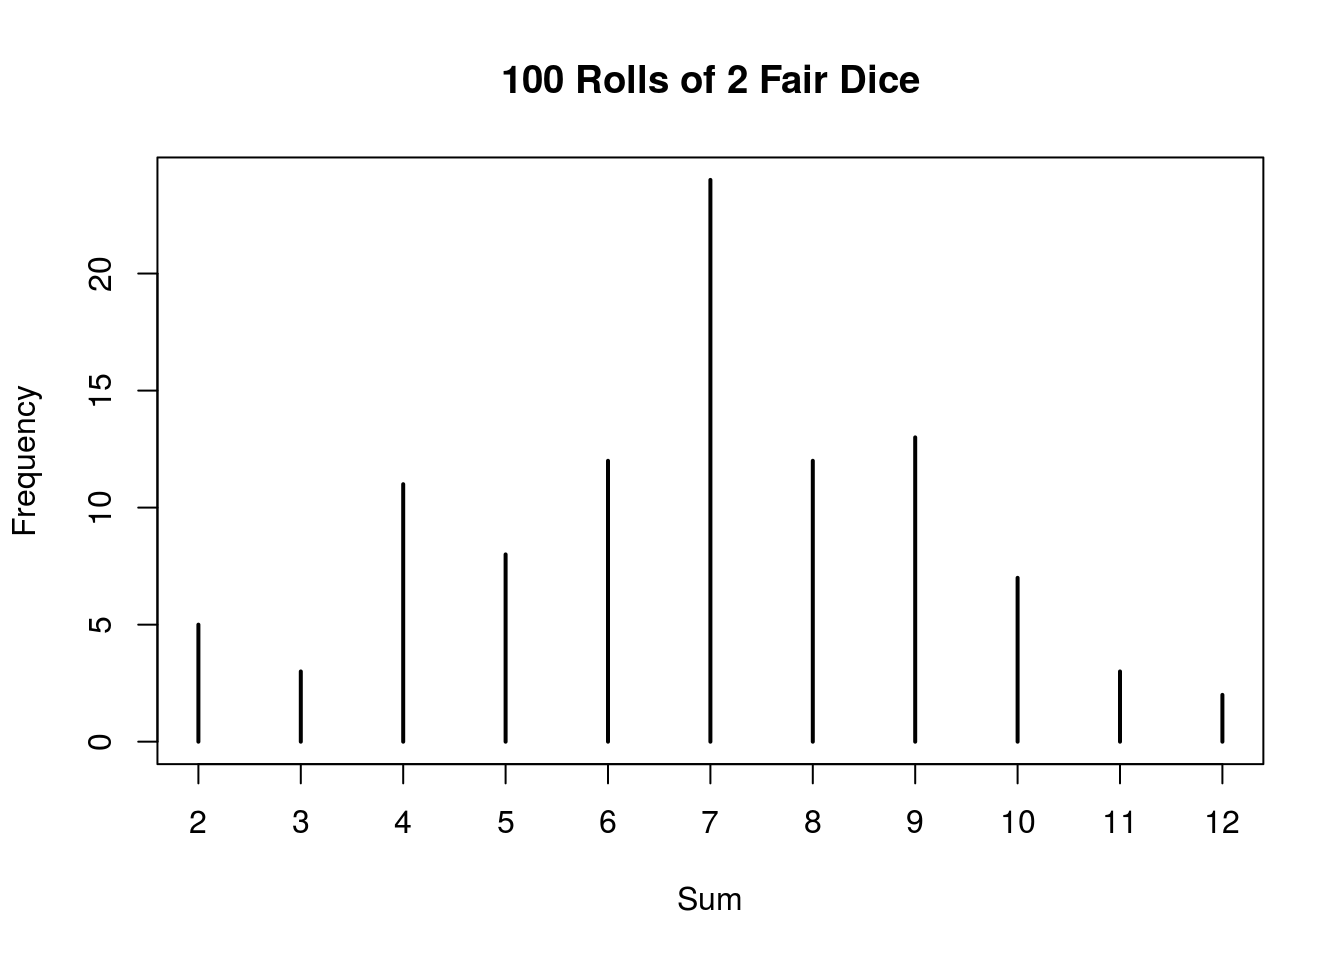
\includegraphics[width=\maxwidth]{figure/unnamed-chunk-30-1} 

}



\end{knitrout}
From this plot, it looks like we need $\Delta$ around 3 in absolute value for the power to be at least 0.5. (Notice that the curve is symmetric.) Let's try a few values:
\begin{knitrout}
\definecolor{shadecolor}{rgb}{0.969, 0.969, 0.969}\color{fgcolor}\begin{kframe}
\begin{alltt}
\hlkwd{power.10}\hlstd{(}\hlnum{3}\hlstd{)}
\end{alltt}
\begin{verbatim}
## [1] 0.5483002
\end{verbatim}
\end{kframe}
\end{knitrout}
So it looks like we can make $\Delta$ even smaller:
\begin{knitrout}
\definecolor{shadecolor}{rgb}{0.969, 0.969, 0.969}\color{fgcolor}\begin{kframe}
\begin{alltt}
\hlkwd{power.10}\hlstd{(}\hlnum{2.7}\hlstd{)}
\end{alltt}
\begin{verbatim}
## [1] 0.4638674
\end{verbatim}
\end{kframe}
\end{knitrout}
Those are too small. Let's try making it a little bigger
\begin{knitrout}
\definecolor{shadecolor}{rgb}{0.969, 0.969, 0.969}\color{fgcolor}\begin{kframe}
\begin{alltt}
\hlkwd{power.10}\hlstd{(}\hlnum{2.75}\hlstd{)}
\end{alltt}
\begin{verbatim}
## [1] 0.4779274
\end{verbatim}
\begin{alltt}
\hlkwd{power.10}\hlstd{(}\hlnum{2.76}\hlstd{)}
\end{alltt}
\begin{verbatim}
## [1] 0.4807434
\end{verbatim}
\begin{alltt}
\hlkwd{power.10}\hlstd{(}\hlnum{2.77}\hlstd{)}
\end{alltt}
\begin{verbatim}
## [1] 0.4835604
\end{verbatim}
\end{kframe}
\end{knitrout}
Notice that because of the symmetry:
\begin{knitrout}
\definecolor{shadecolor}{rgb}{0.969, 0.969, 0.969}\color{fgcolor}\begin{kframe}
\begin{alltt}
\hlkwd{power.10}\hlstd{(}\hlopt{-}\hlnum{2.77}\hlstd{)}
\end{alltt}
\begin{verbatim}
## [1] 0.4835604
\end{verbatim}
\end{kframe}
\end{knitrout}
Thus, in order to have at least a 50\% of rejecting the null with a sample size of 10, the true difference of means needs to be \emph{at least} 2.77 in absolute value. This is quite a large difference relative to the population standard deviations!

Finally, let's evaluate the power when $\Delta = 0$:
\begin{knitrout}
\definecolor{shadecolor}{rgb}{0.969, 0.969, 0.969}\color{fgcolor}\begin{kframe}
\begin{alltt}
\hlkwd{power.10}\hlstd{(}\hlnum{0}\hlstd{)}
\end{alltt}
\begin{verbatim}
## [1] 0.04550026
\end{verbatim}
\end{kframe}
\end{knitrout}
We get 0.05, which is the significance level of the test! (The only reason it is not exactly equal to 0.05 is that we rounded the critical value for our test to 2. 
The reason this happens is that when $\Delta = 0$ the null is \emph{true}. In hypothesis testing, we set everything up so the probability of rejecting a true null equals $\alpha$.
      \end{solution}
			\part Repeat parts (a) and (b) with $n = m = 100$. How do your results change? Explain.
        \begin{solution}
        We can use the same procedure as above. The only difference is the standard error used in the test statistic. Whereas before this was $\sqrt{2}$, now we have:
        $$SE = \sqrt{\sigma_X^2/n + \sigma_Y^2/m} = \sqrt{10/100 + 10/100} = \sqrt{1/5} = 1/\sqrt{5}$$
    Thus, putting $1/\sqrt{5}$ in place of $\sqrt{2}$, we have
    $$\mbox{Power}(\Delta) = \texttt{pnorm}(-2 - \Delta\sqrt{5}) + \left[1 - \texttt{pnorm}(2 - \Delta\sqrt{5})\right]$$  
\begin{knitrout}
\definecolor{shadecolor}{rgb}{0.969, 0.969, 0.969}\color{fgcolor}\begin{kframe}
\begin{alltt}
\hlstd{power.100} \hlkwb{<-} \hlkwa{function}\hlstd{(}\hlkwc{delta}\hlstd{)\{}
  \hlstd{greater} \hlkwb{<-} \hlnum{1} \hlopt{-} \hlkwd{pnorm}\hlstd{(}\hlnum{2} \hlopt{-} \hlstd{delta} \hlopt{*} \hlkwd{sqrt}\hlstd{(}\hlnum{5}\hlstd{))}
  \hlstd{less} \hlkwb{<-} \hlkwd{pnorm}\hlstd{(}\hlopt{-}\hlnum{2} \hlopt{-} \hlstd{delta} \hlopt{*} \hlkwd{sqrt}\hlstd{(}\hlnum{5}\hlstd{))}
  \hlstd{power} \hlkwb{<-} \hlstd{greater} \hlopt{+} \hlstd{less}
  \hlkwd{return}\hlstd{(power)}
\hlstd{\}}
\end{alltt}
\end{kframe}
\end{knitrout}
We can compare this to the power function when $n=m=10$ by plotting them on the same graph as follows:
\begin{knitrout}
\definecolor{shadecolor}{rgb}{0.969, 0.969, 0.969}\color{fgcolor}\begin{kframe}
\begin{alltt}
\hlstd{y} \hlkwb{<-} \hlkwd{cbind}\hlstd{(}\hlkwd{power.10}\hlstd{(delta),} \hlkwd{power.100}\hlstd{(delta))}
\hlkwd{matplot}\hlstd{(delta, y,} \hlkwc{type} \hlstd{=} \hlstr{'l'}\hlstd{,} \hlkwc{ylab} \hlstd{=} \hlstr{'Power'}\hlstd{,} \hlkwc{col} \hlstd{=} \hlkwd{c}\hlstd{(}\hlstr{'blue'}\hlstd{,} \hlstr{'red'}\hlstd{),} \hlkwc{lty} \hlstd{=} \hlnum{1}\hlstd{)}
\end{alltt}
\end{kframe}

{\centering 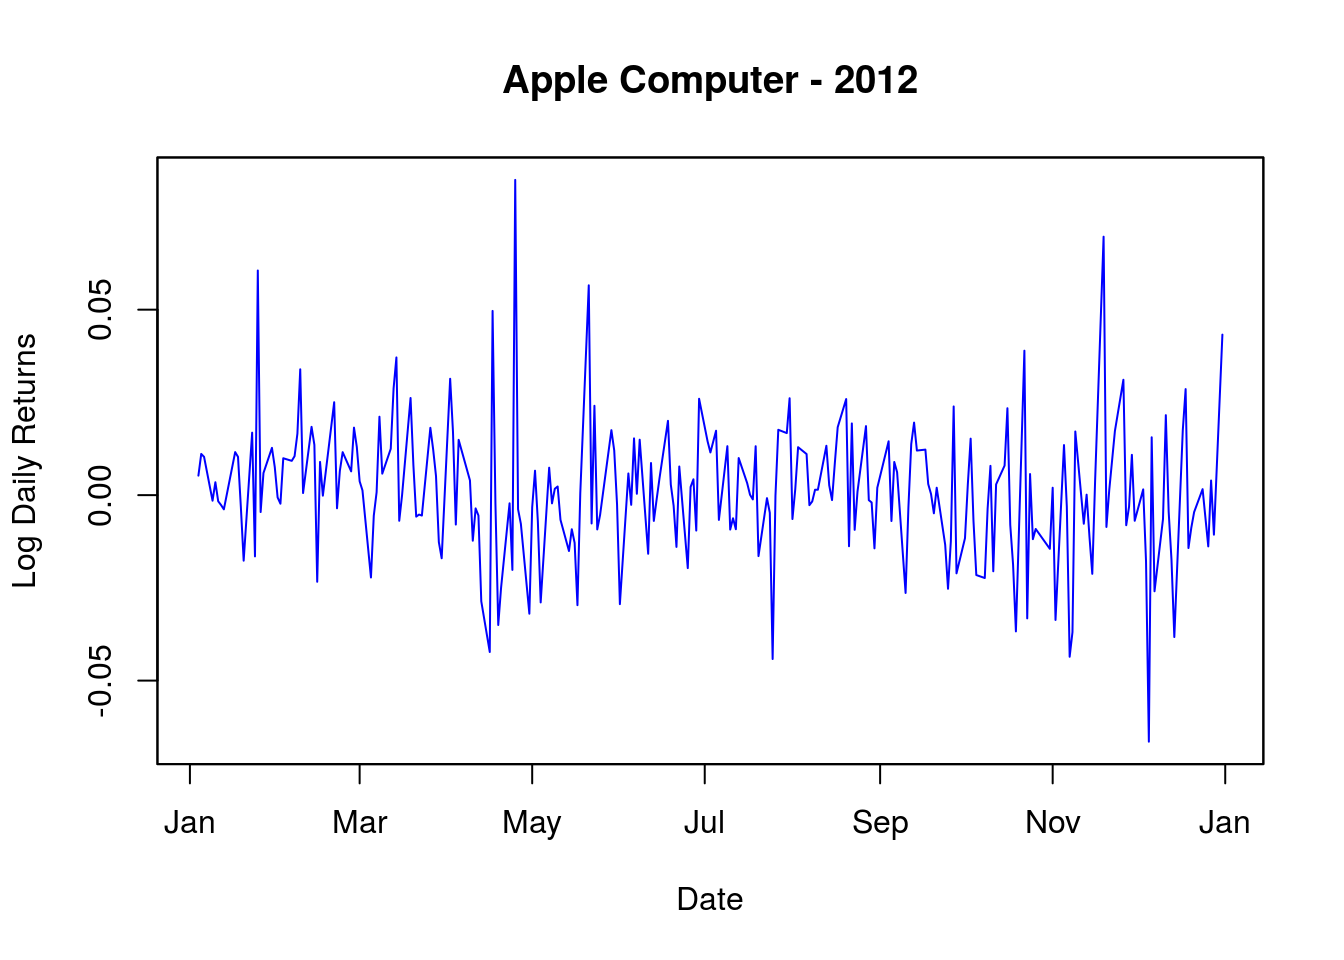
\includegraphics[width=\maxwidth]{figure/unnamed-chunk-37-1} 

}



\end{knitrout}
where the red curve is $n = m = 100$ and the blue curve is $n=m=10$. We see that for any value of $\Delta$, power is higher for the test based on a larger sample size: we are more likely to detect a difference of a given size using large samples. 

Experimenting with \texttt{power.100} as we did above for \texttt{power.10}, 
\begin{knitrout}
\definecolor{shadecolor}{rgb}{0.969, 0.969, 0.969}\color{fgcolor}\begin{kframe}
\begin{alltt}
\hlkwd{power.100}\hlstd{(}\hlnum{1}\hlstd{)}
\end{alltt}
\begin{verbatim}
## [1] 0.5933214
\end{verbatim}
\begin{alltt}
\hlkwd{power.100}\hlstd{(}\hlnum{0.9}\hlstd{)}
\end{alltt}
\begin{verbatim}
## [1] 0.5050012
\end{verbatim}
\begin{alltt}
\hlkwd{power.100}\hlstd{(}\hlnum{0.89}\hlstd{)}
\end{alltt}
\begin{verbatim}
## [1] 0.4960838
\end{verbatim}
\begin{alltt}
\hlkwd{power.100}\hlstd{(}\hlnum{0.88}\hlstd{)}
\end{alltt}
\begin{verbatim}
## [1] 0.4871686
\end{verbatim}
\end{kframe}
\end{knitrout}
So it looks like we need a difference between the two population means of at least 0.88 (in absolute value) to have at least a 50\% chance of rejecting the null of no difference. Notice that this is a much smaller difference than we needed above (2.77) because of the increased sample size. 

Finally, as above, if $\Delta = 0$ then the null is true, and the probability of rejecting a \emph{true} null is simply $\alpha$
\begin{knitrout}
\definecolor{shadecolor}{rgb}{0.969, 0.969, 0.969}\color{fgcolor}\begin{kframe}
\begin{alltt}
\hlkwd{power.100}\hlstd{(}\hlnum{0}\hlstd{)}
\end{alltt}
\begin{verbatim}
## [1] 0.04550026
\end{verbatim}
\end{kframe}
\end{knitrout}
Again, there's only a slight difference from the exact value of 0.05. This is because we rounded the critical value for our test to 2. 
        \end{solution}
	\end{parts}


\question  Professor Neil is interested in determining whether viewing different colors affects subjects' mental states in a way that alters their athletic ability. As a part of her research she carries out the following experiment. Each subject is randomly assigned to wait in one of two rooms: a room in which all of the walls have been painted pink or another in which all of the walls have been painted red. After waiting for five minutes, each subject is taken to a track and asked to run a 5K as fast as possible. Using the data from this experiment, Professor Neil carries out a statistical test of the null hypothesis that the population mean 5K time is equal across groups (those who waited in the pink room versus those who waited in the red room). Testing at the 1\% level, she finds a statistically significant difference. For each of the following, answer True or False. If false, explain.
	\begin{parts}
		\part The p-value for the null hypothesis that population means are equal across groups is greater than 0.01.
			\begin{solution}
			False: the p-value is \emph{less than or equal to} 0.01. 
			\end{solution}
		\part Professor Neil would also have found a statistically significant difference had she carried out her test at the 5\% level.
		\begin{solution}
		True.
		\end{solution}
		\part If there were really no difference in population means across the two groups, the chance of observing a test statistic at least as extreme as that observed by Professor Neil would be 0.01 or less.
		\begin{solution}
		True.
		\end{solution}
		\part Professor Neil's findings have important practical implications for sports regulatory organizations such as the International Olympic Committee: all locker rooms should be painted exactly the same color to keep from throwing off the outcomes of sporting events.
			\begin{solution}
			False. Professor Neil has found strong evidence of a difference in population means across the two groups. However, none of the information given above provides any indication of whether this difference is large enough to have any practical importance. In the words of the textbook ``statistical significance and practical significance are two entirely different matters.'' For example, the difference of population means could be one second. This is far too small to be likely to change the outcome of a 5K race, but with a large enough sample size we would still be able to detect it. Unlike a confidence interval, which gives us a range of plausible values for the difference in population means, a hypothesis test merely tells us whether we have strong evidence that a difference exists. 
			\end{solution}
	\end{parts}



\end{questions}


\end{document}
